\chapter{Improved Initial Data for Spinning Binary Neutron Stars}

\section{Chapter Overview}
This is a set of notes regarding a bug found the code we use to
generate initial data for spinning binary neutron stars.

\section{Introduction}
Recently, \cite{Tacik:2015tja} presented results for the
construction and evolution of binary neutron stars with arbirary spin
vectors using the SpEC code. In this chapter, we will revisit those
results. Namely we have found a computational error in the code that
was used to generate those results. We will begin by discussing what
the error was and what the general implications of that are. We will
then revisit and update the results of \cite{Tacik:2015tja} in lieu of
this. Finally, we will then discuss how the results of
\cite{Tacik:2015tja} can be pushed even further.

\section{Erroneuous code}
\begin{verbatim}
	Dm b1(sd,0.0);
	for (int i=0;i<3;i++){
	  b1 += Shift(i)*moddPot(i);
	}
	b1 = sqr(b1 + CEuler);

	Dm b2(sd,0.0);
	for (int i=0;i<3;i++){
	  for (int j=0;j<3;j++){
	    b2 += Invg(i,j)/(sqr(sqr(Psi)))*(moddPot(i)+Rot(i))*Rot(j);
	  }
	}

	Dm H = sqr(b1) + 2*b1*b2;
	H = sqrt(H);
	H += (b1+b2);
	H = H / (2*sqr(Lapse));
	
	for (int i =0; i <3; i++){
	  for (int j=0; j<3; j++){
	    H -= Invg(i,j) / (sqr(sqr(Psi))) * (moddPot(i)) * (moddPot(j));
	  } 
	}
	H = sqrt(H);
\end{verbatim}

\section{Revised Code}
\begin{verbatim}
	Dm b1(sd,0.0);
	for (int i=0; i<3; i++){
	  b1 += Shift(i)*moddPot(i);
	}
	b1 = sqr(b1 + CEuler);

	Dm b2(sd,0.0);
	for (int i=0; i<3; i++){
	  for (int j=0; j<3; j++){
	    b2 += Invg(i,j) / (sqr(sqr(Psi))) * (moddPot(i)+Rot(i)) * Rot(j);
	  }
	}
	b2 *= (2 * Lapse * Lapse);

	Dm L2(sd, 0.0);
	L2 = ((b1+b2) + sqrt(sqr(b1)+2*b1*b2))/(2*sqr(Lapse));
	
	Dm H = L2;
	for (int i=0; i <3; i++){
	  for (int j=0; j<3; j++){
	    H -= Invg(i,j)/(sqr(sqr(Psi))) * (moddPot(i)+Rot(i))*(moddPot(j)+Rot(j));
	  }
	}
	H = sqrt(H);
\end{verbatim}

\section{Description of Bug}
Following~\cite{Tichy:2012rp}, the 3-velocity of the neutron star fluid in an
inspiralling binary is written as the sum of an irrotational part and
a rotational part:
\begin{equation}
U^i =
\frac{\Psi{-4}\tilde{\gamma}^{ij}}{h\gamma_n}\left(\partial_j\phi +
  W_j\right).
\end{equation}
Here $\Psi$ is the conformal factor, $\tilde{\gamma}_{ij}$ is the
conformal metric, $h$ is the specific enthalpy, $\gamma_n$ is the
Lorentz term $\gamma_n=\left(1-\gamma_{ij}U^iU^j\right)^{-1/2}$,
$\phi$ is the irrotational velocity potential, and $W$ is the rotation
term, designed to endow a uniform rotation to the star. In this
construction, the solution of the Euler equation is
\begin{equation}
h=\sqrt{L^2-\left(\nabla_i\phi+W_i\right)\left(\nabla^i\phi+W^i\right)}
\end{equation}
where
\begin{equation}
L^2 = \frac{(x+y)+\sqrt{x^2+2xy}}{2\alpha^2}
\end{equation}
\begin{equation}
x=\left(\beta^i\nabla_i\phi+C\right)^2
\end{equation}
\begin{equation}
y=2\alpha^2\left(\nabla_i+W_i\right)W^i
\end{equation}
However, our code indicates that we have computed the following
quantity instead
\begin{equation}
h'=\sqrt{L^2-\left(\nabla_i\phi\right)\left(\nabla^i\phi\right)}
\end{equation}
where 
\begin{equation}
y'=\left(\nabla_i\phi+W_i\right)W^i
\end{equation}
The difference between the two quantities is
\begin{equation}
h'^2-h^2 =
\frac{\left(y'-y\right)}{2\alpha^2}+\frac{\sqrt{x^2+2xy}-\sqrt{x^2+2xy'}}{2\alpha^2}-W_iW^i-\nabla_i\phi\left(\nabla^i\phi+W^i\right)
\end{equation}
Let's take a rough limit where $W$ is very large and only consider
terms of order $W^2$.
Then this difference is 
\begin{equation}
h'^2-h^2 = \frac{W^2\left(1-4\alpha^2\right)}{2\alpha^2}
\end{equation}
Since $\alpha$ should generally be $>0.5$, this will be a negative
number. This means that the enthalpy was too low, which means the
density was too low, which means it wants to increase. This is what is
seen in our simulations.

\section{Revisiting previous results}
Having re-coded the erroneous code, we now revisit the results of \cite{Tacik:2015tja}.

\subsection{Size of density oscillations}
We constructed initial data with the same input files as for the S0.4z
run of \cite{Tacik:2015tja}, and evolved it with the same input files
as well, for about $2500M_{\odot}$. In figure ~\ref{fig:NewS4Density}
we plot the normalized density oscillations ($\rho / \rho(t=0)$, where
$\rho$ represents the maximum density) for both cases. We see that
previously the peak-to-peak density oscillations were about $20\%$,
whereas now they are about $0.5\%$, a decrease by about a factor of
40. This is in line with what is seen in simulations of non-spinning
binary neutron stars (R. Hass, Priv. comm). The period of oscillation remains the same as it was previously,
indicating that it probably still represents an excited quasi-normal mode oscillation. We note now, however, that the phase of oscillation has changed by approximately half of a period.

\begin{figure}[!ht]
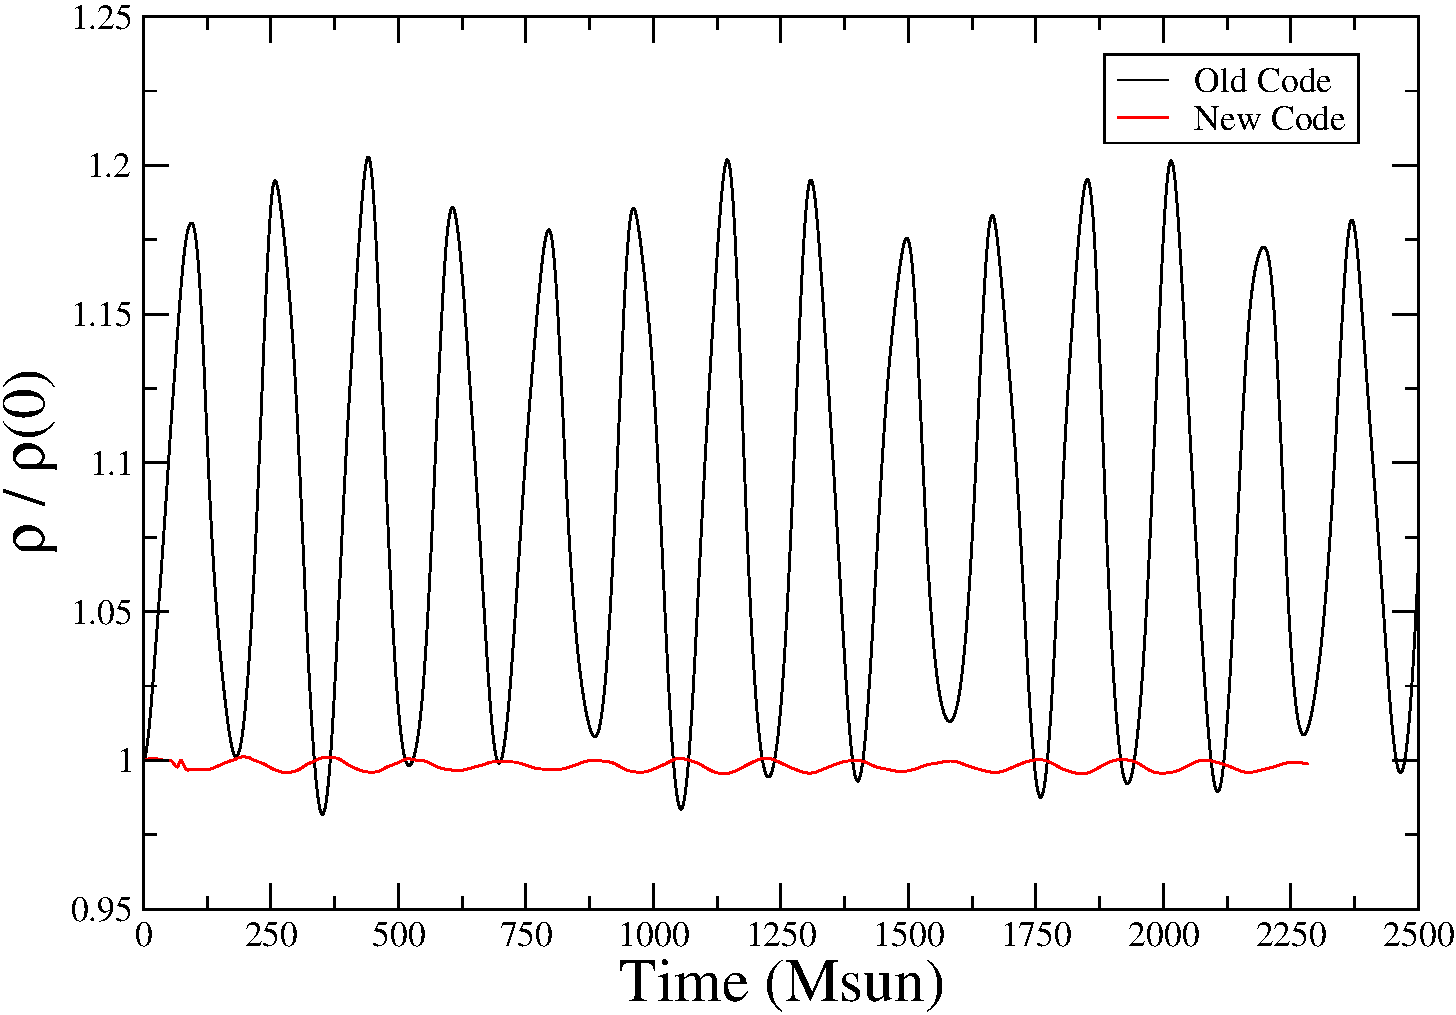
\includegraphics[width=0.95\columnwidth]{chap6/NewS4Density}
\caption{\label{fig:NewS4Density} Normalized density oscillations for
  the S0.4z run from \cite{Tacik:2015tja} and from a new run with the same
parameters.}
\end{figure}

\subsection{Magnitude of spin}
With a change in the computation of the enthalpy, and thus
distribution of the equilibrium enthalpy, the spin of the star may
change. In particular, in the old bugged code, the starting radius of
the star was too large (the density too small) and the oscillations
would begin. Since $\chi \propto R^2$, we would expect that the
dimensionless spin show be higher in the old code. In
figure~\ref{fig:NewS4Spin} we plot the spin during the evolution,
measured in the way described in~\cite{Tacik:2015tja}, for the new
and old codes. Indeed we see that dimensionless spin has descreased
from $\sim 0.375$ to $\sim 0.33$. Similar to the case of the density
oscillations, the spin oscillations are still present in the new code,
but they are much lower in magnitude and are half a period out of
phase with the previous data.

\begin{figure}[!ht]
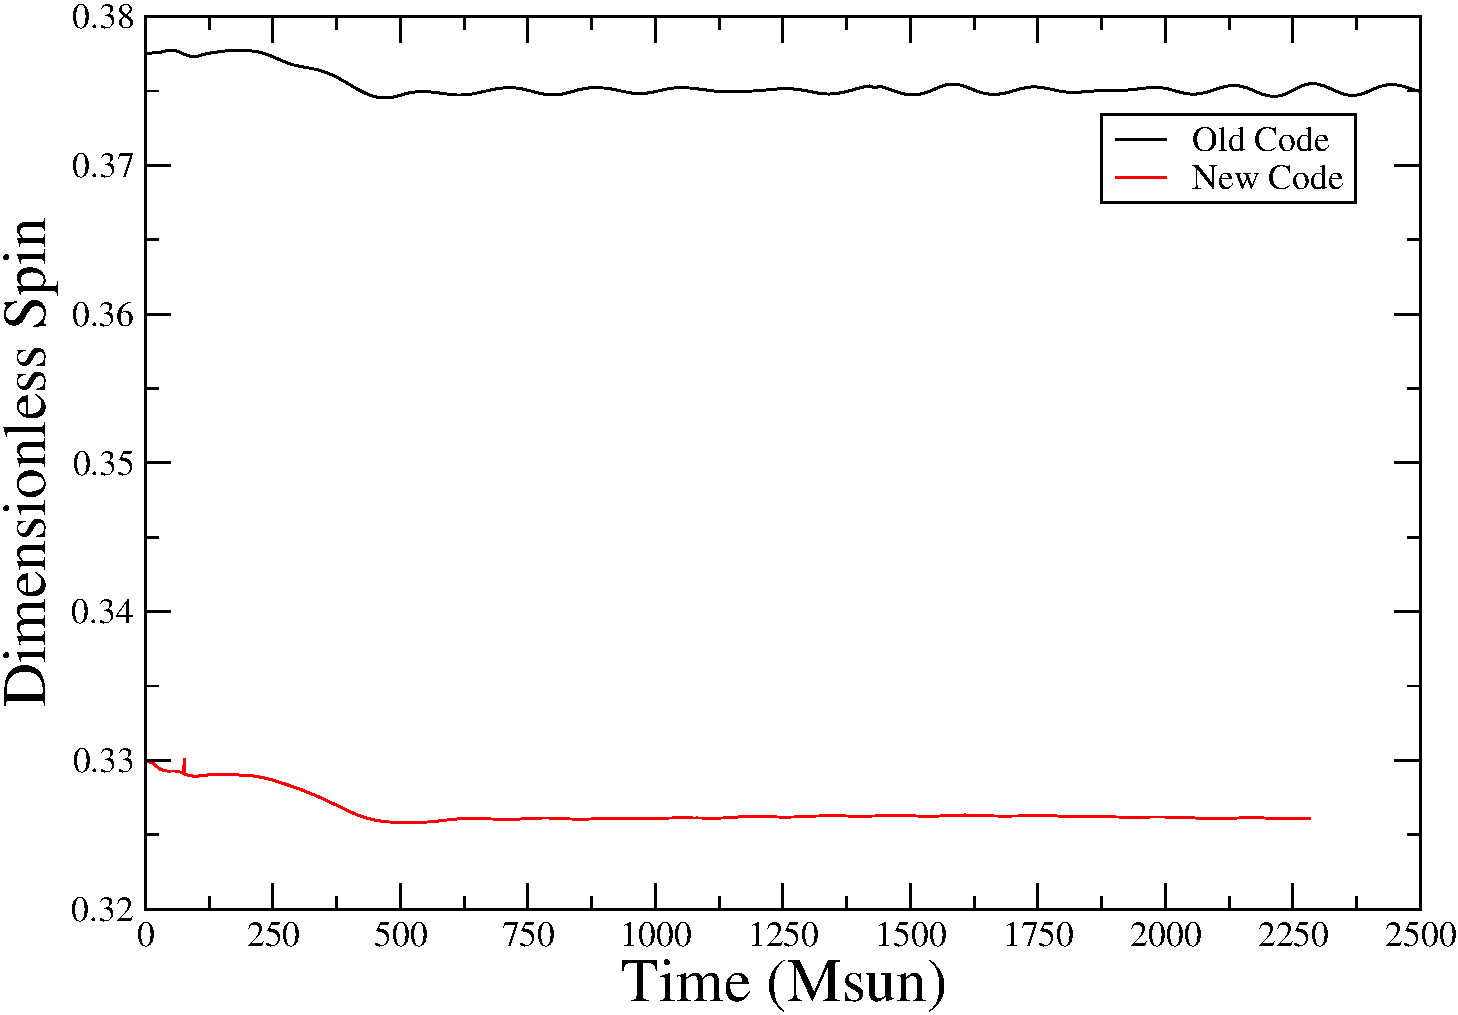
\includegraphics[width=0.95\columnwidth]{chap6/NewS4Spin}
\caption{\label{fig:NewS4Spin} Dimensionless spin,
  $\chi=\frac{J}{M_{\rm ADM}^2}$, measured during the
  evolution of the S0.4z run from~\cite{Tacik:2015tja} with the old
  code and the new code.}
\end{figure}

\subsection{$\chi - \Omega$ relation}
As we have just seen, the new computation of the enthalpy means that
the $\chi(\Omega)$ relation is changed. Thus we will now re-visit Fig. 8 of
\cite{Tacik:2015tja} where $\chi$ is plotted as a function of
$\Omega$. First, we re-compute all the initial data sets as before
with the same values of $\Omega$. However, because our computation is
now more robust, we are also able to extend to much higher values of
$\Omega$ than before. Therefore, we also use this plot to explore how
much higher the initial data solver can be pushed.  The new relation
is shown in figure~\ref{fig:NewChiVOmega}. 
\begin{figure}[!ht]
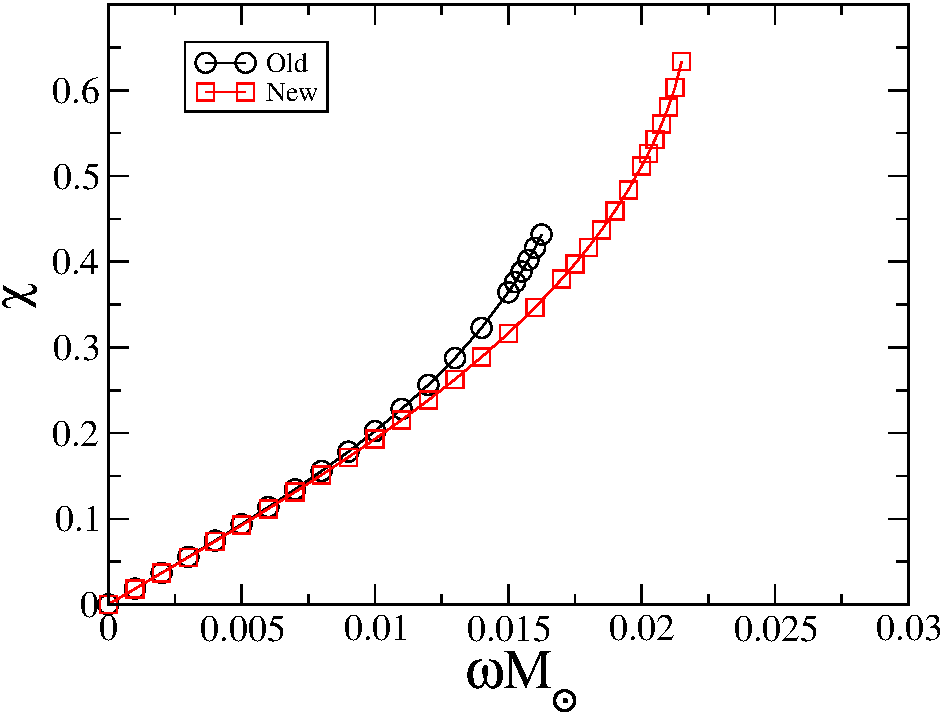
\includegraphics[width=0.95\columnwidth]{chap6/NewChiVOmega}
\caption{\label{fig:NewChiVOmega} $\chi$ as a function of $\Omega$ in
  the initial data. The black curve is from Fig. 8 of
  \cite{Tacik:2015tja}, while the red curve is generated with the bug fixed.}
\end{figure}
First, we note that the $\chi(\Omega)$ relation is unchanged at low
values of $\Omega$. In  \cite{Tacik:2015tja}, a value of
$|\Omega|=0.00273$ was used for the S-0.05z run - so it is probably
unaffected significantly by this bug. Second, we note that the new
curve is indeed below the old curve, as predicted above. Finally, we
note that the initial data solver can indeed be pushed much further
now. Before it was able to reach spins of $\sim 0.43$, and now it can
reach spins of $\sim 0.63$ - quite a significant increase. This $0.63$
is in fact above the theoretical $0.57$ limit quoted
in~\cite{Ansorg:2003br}, and more in line with the values from studies
like ~\cite{Lo:2010bj}. Clearly this invites further investigation.

\subsection{Initial Data Convergence}
We'll know look at how the changed enthalpy computation affects the convergence of the initial data. Again, we focus on the S0.4z run from \cite{Tacik:2015tja} using the same input files. In figure ~\ref{fig:NewS4HamMom} we look at the Hamiltonian and Momentum constraints for the new code. We do not find a very significant difference between the two. Presumably this is because many there are many factors that affect the constraints. Furthermore, we were previously still solving the field equations correctly, it just happened to be for a star that was out of equilirbium.

\begin{figure}[!ht]
\includegraphics[width=0.95\columnwidth]{chap6/NewHamMom}
\caption{\label{fig:NewS4HamMom} Hamiltonian and Momentum constraints
  for the new and old code, for the S0.4z run.}
\end{figure}

Next, we look at how the global quantities $E_{\rm ADM}$ and $J_{\rm
  ADM}$ are affected by this computational change. This is plotted in
Fig.~\ref{fig:EADMConvergence}. In particular we are plotting the
fractional difference between adjacent resolutions as a function of
the lower resolution. The ``old''' data is from Fig.5 of \cite{Tacik:2015tja}. Again, there does not seem to be a
large change here (although the $E_{\rm ADM}$ slope for the new
initial data is much more shallow and the data start much lower at low resolution.

\begin{figure}[!ht]
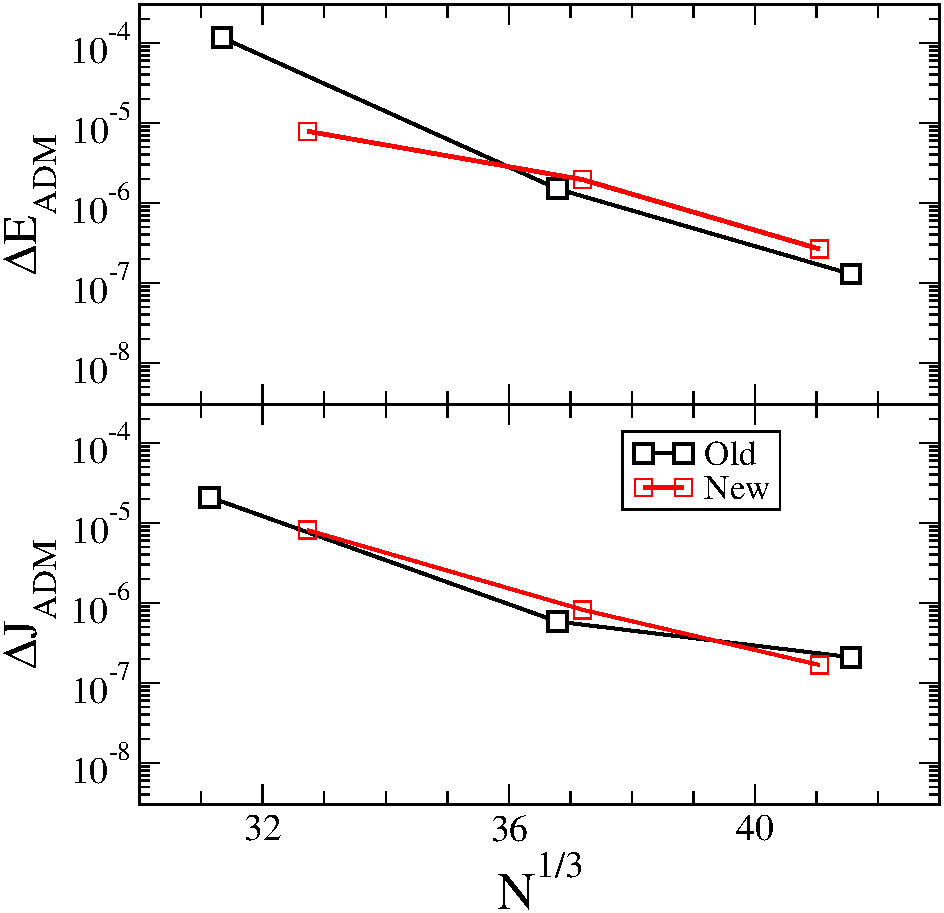
\includegraphics[width=0.95\columnwidth]{chap6/EADMConvergence}
\caption{\label{fig:EADMConvergence} Fractional convergence of the ADM
energy and ADM angular momentum for the new and old codes.}
\end{figure}

Next, we look how the spin in the initial data convergences with
resolution. This is plotted in figure~\ref{fig:NewSpinConvergence}. In
particular we plot the absolute difference between $\chi(N)$ and
$\chi$ at the highest resolution. The ``old'' data is from Fig. 6 of
\cite{Tacik:2015tja}. The new data seems to be lower than the old data
by a fairly significant amount.

\begin{figure}[!ht]
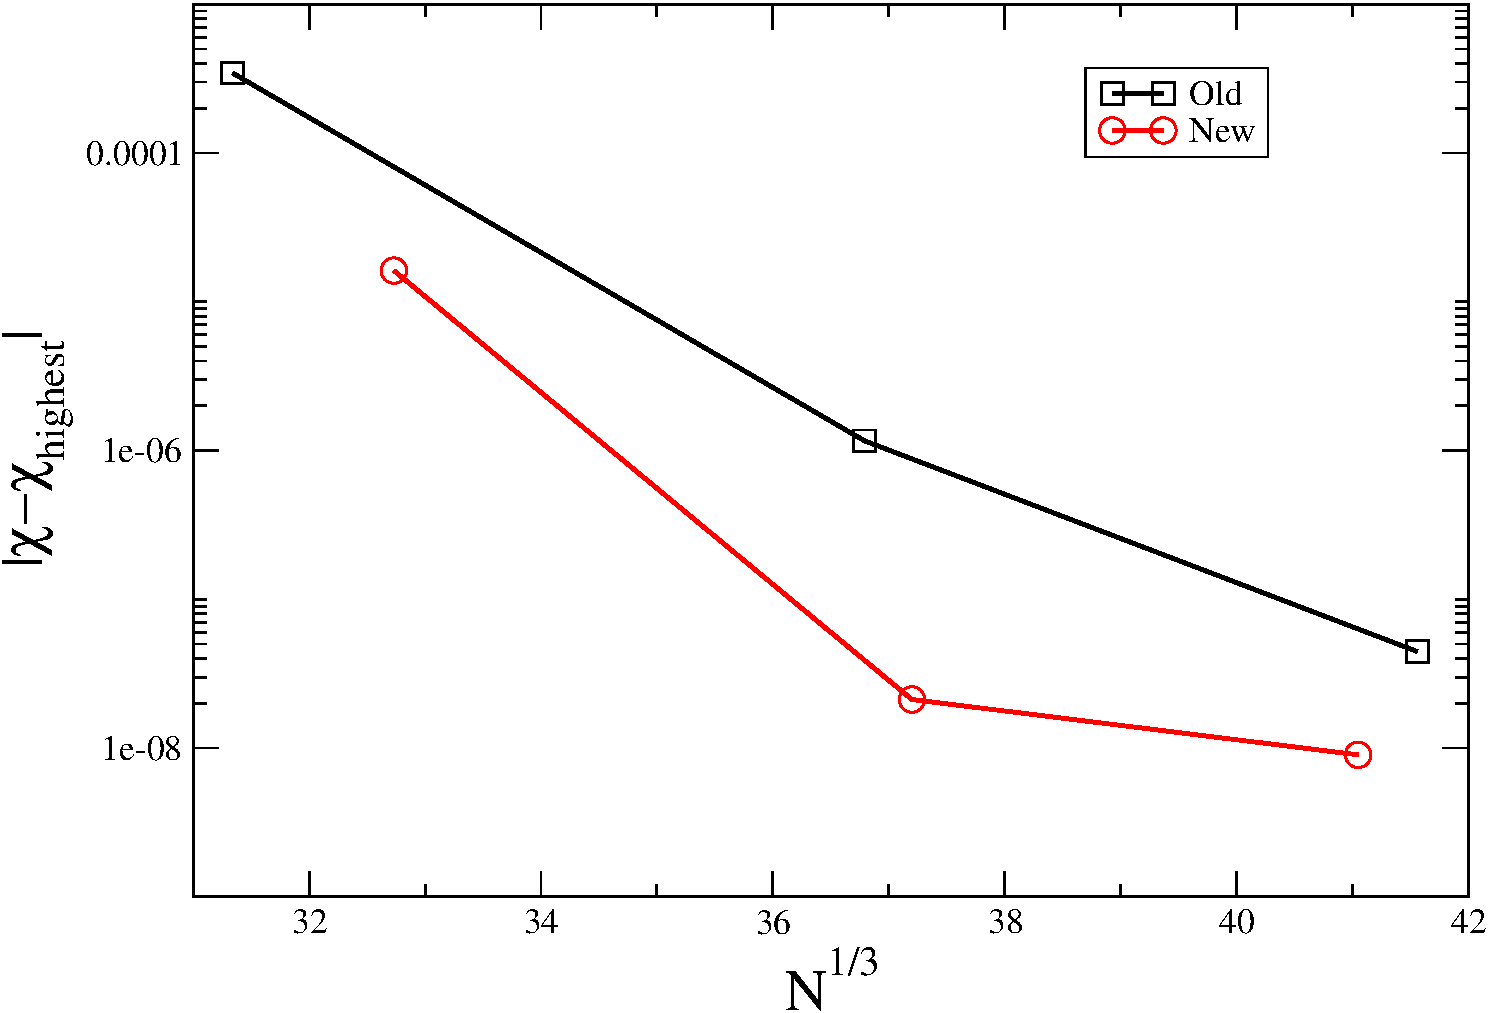
\includegraphics[width=0.95\columnwidth]{chap6/NewSpinConvergence}
\caption{\label{fig:NewSpinConvergence} Convergence of the spin
  measured in the initial data for the new and old codes.}
\end{figure}

\subsection{Komar Mass}
As noted in~\cite{FoucartEtAl:2008}, the difference between the Komar mass $M_K$ and the
ADM energy $M_{\rm ADM}$ is an indicator of deviations from
equilibrium. We now suspect our neutron star is more close to being in
equilibirum, and therefore except that this difference would be
smaller. Let us investigate this. We again look at the same S0.4z
comparison. In the old results, at the highest initial data
resolution, this difference is $|(M_K-M_{\rm ADM})/M_k \sim 2.6 \times
10^{-3}$. In the new results, this difference is 
$|(M_K-M_{\rm ADM})/M_k \sim 2.1 \times
10^{-4}$. So indeed, this difference has decreased by more than an
order of magnitude.

\section{Higher Spin Evolutions}
As shown in Fig.~\ref{fig:NewChiVOmega}, the initial data solver can
now construct initial data for much higher spins than before. Let us
try to evolve some of these.

\subsection{Evolution 1}
Here we construct and evolve initial data with $\Omega=0.019\hat{z}$. In
figure~\ref{fig:Ev1Snapshot} we present a snapshot of the run,
plotting the normalized density oscillations, measured spin, and the
orbit of the stars. The dimensionless spin is about $\chi \sim
0.46$. The peak-to-peak density oscillations are now about
$2\%$. Higher than in the previous evolution, but still much smaller
than in \cite{Tacik:2015tja}. We have performed about three orbits of evolution.

\begin{figure}[!ht]
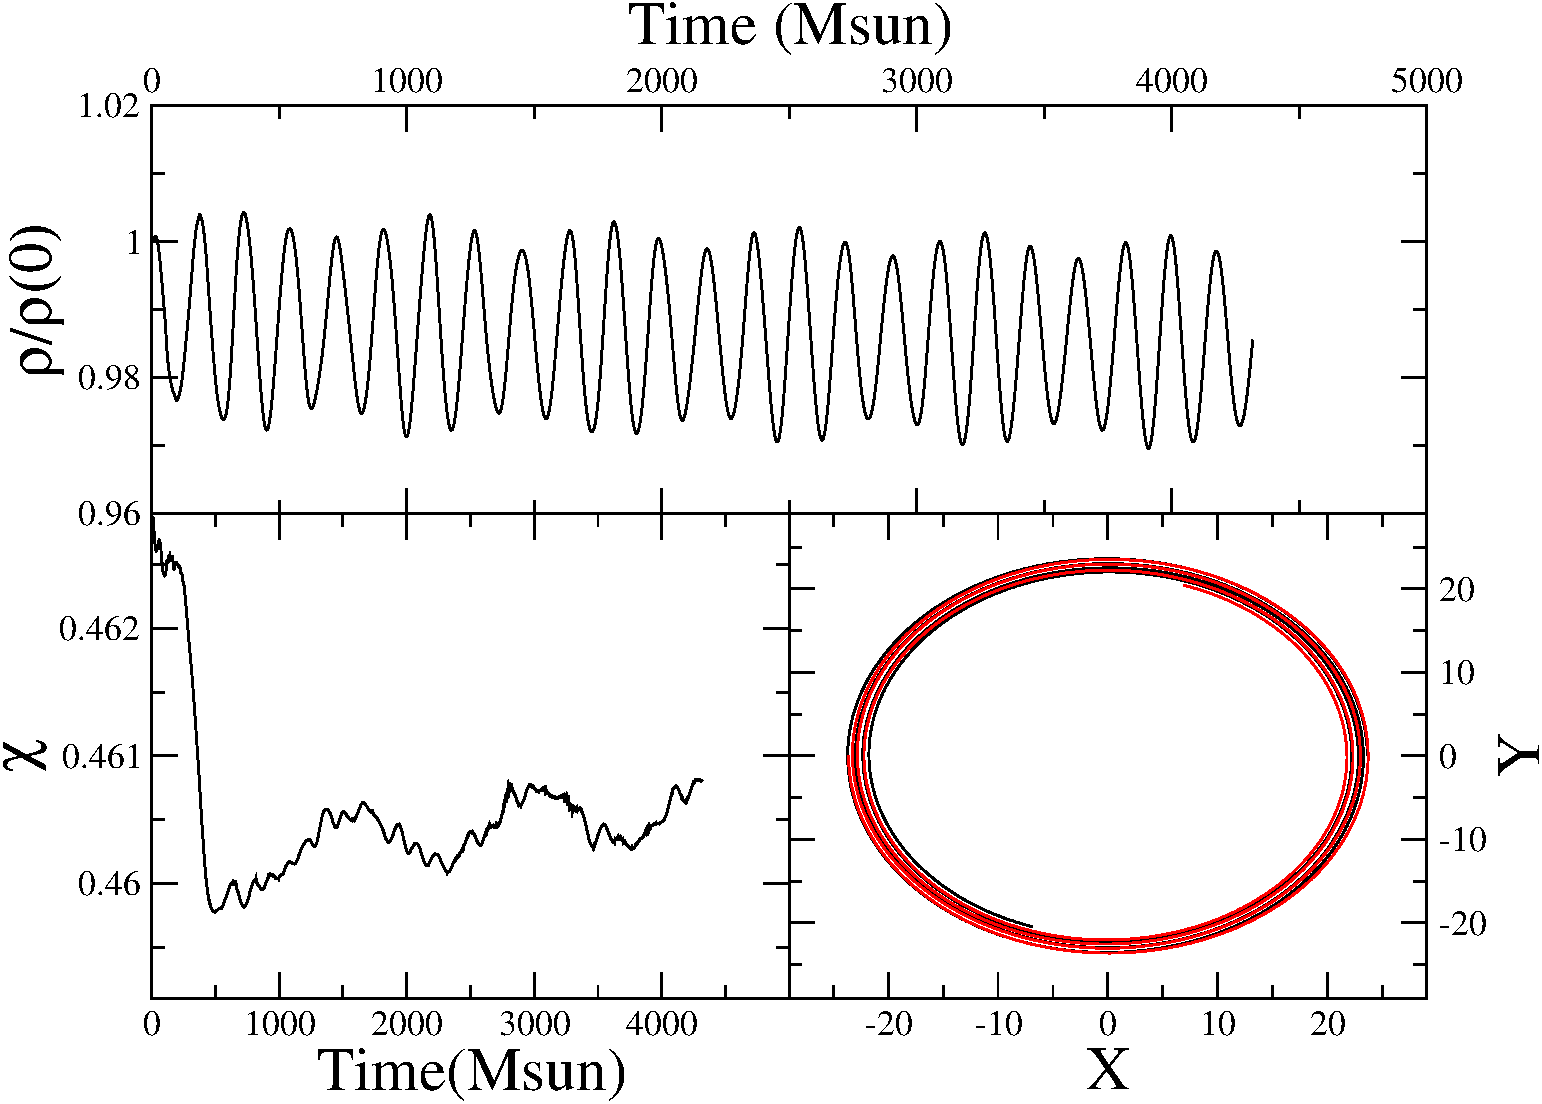
\includegraphics[width=0.95\columnwidth]{chap6/Ev1Snapshot}
\caption{\label{fig:Ev1Snapshot} A snapshot of an evolution with
  $\Omega=0.019$. The top panel shows the normalized density
  oscillations. The bottom-left panel shows the measured spin of a
  star. The bottom-right panel shows the orbtis of the stars as they
  inspiral.}
\end{figure}

\subsection{Evolution 2}
Here we construct and evolve initial data with $\Omega=0.0215\hat{z}$. The
evolution has only recently begun so we can only make tentative
conclusions. But the peak-to-peak density oscillations are around
$6\%$, and the spin during the evolution is around $\chi\sim0.625$. See
Fig.~\ref{fig:Ev2Snapshot}.

\begin{figure}[!ht]
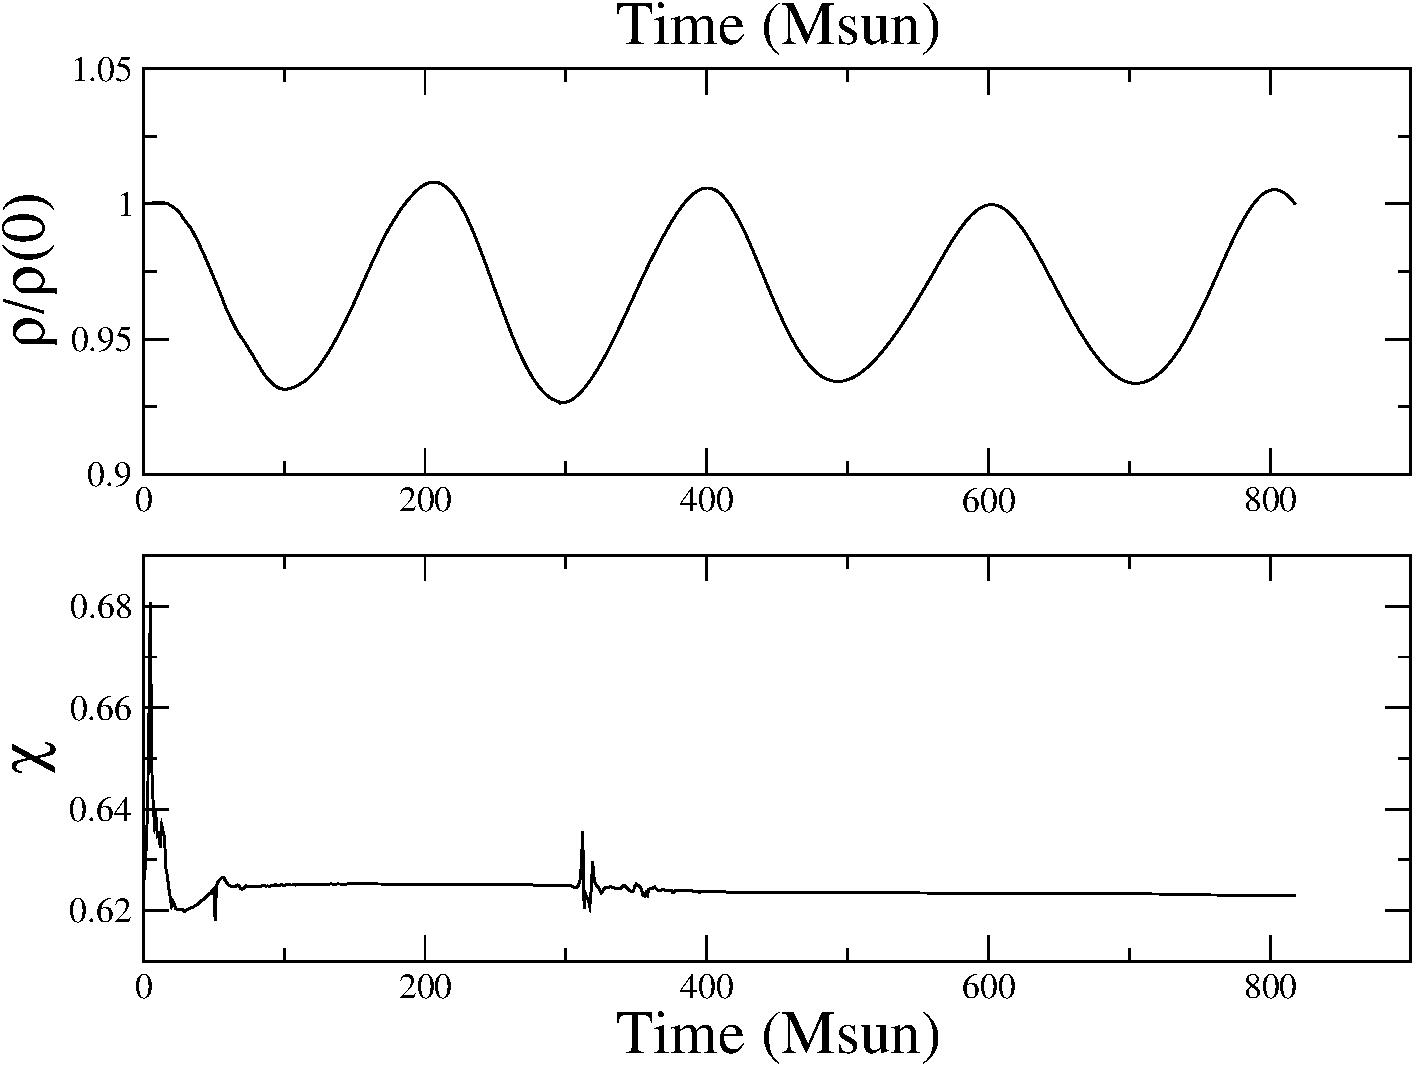
\includegraphics[width=0.95\columnwidth]{chap6/Ev2Snapshot}
\caption{\label{fig:Ev2Snapshot} Density oscillations and and measured
  spin for evolution 2. This run has only recently begun.}
\end{figure}

%\section{Conclusion}
%Concluding remarks
